\documentclass[10pt,letterpaper]{article}
\usepackage[margin=.85in]{geometry}
\usepackage[T1]{fontenc}
\usepackage{lmodern,microtype,amsmath,amssymb}
\usepackage{booktabs,array,longtable,tabularx,enumitem}
\usepackage{xcolor,tikz,hyperref,xurl,fancyhdr,needspace}
\usetikzlibrary{arrows.meta,positioning,calc}
\definecolor{ink}{HTML}{183448}
\definecolor{accent}{HTML}{245D73}
\definecolor{pale}{HTML}{EFF5F7}
\hypersetup{colorlinks=true,linkcolor=accent,urlcolor=accent,citecolor=accent,
  pdftitle={TriAlign Technical Design and Research Notes},
  pdfauthor={Jonathan Ma and Jiatong Gao}}
\setlist[itemize]{leftmargin=1.6em,itemsep=.25em,topsep=.4em}
\setlist[enumerate]{leftmargin=1.9em,itemsep=.35em,topsep=.4em}
\setlength{\parskip}{.35em}
\setlength{\parindent}{0pt}
\setlength{\emergencystretch}{2em}
\renewcommand{\arraystretch}{1.18}
\newcolumntype{L}[1]{>{\raggedright\arraybackslash}p{#1}}
\newcolumntype{Y}{>{\raggedright\arraybackslash}X}
\newcommand{\code}[1]{\texttt{\detokenize{#1}}}
\newcommand{\pathcode}[1]{\nolinkurl{#1}}
\newcommand{\planned}{\textit{Proposed design.}}
\newcommand{\research}{\textit{Research note; adaptation not yet implemented or evaluated.}}
\pagestyle{fancy}
\fancyhf{}
\fancyhead[L]{\small\textcolor{ink}{TriAlign technical design}}
\fancyhead[R]{\small November 2026}
\fancyfoot[C]{\thepage}
\setlength{\headheight}{14pt}
\setcounter{tocdepth}{2}
\title{\textcolor{ink}{TriAlign Technical Design}\\[.4em]
  \large Clinical-Meaning Comparison of Trial Eligibility Criteria\\
  \normalsize Architecture, Dataset, Pair Semantics, Interface Concepts, and Research Notes}
\author{Jonathan Ma \and Jiatong Gao}
\date{November 1, 2026}

\begin{document}
\maketitle
\begin{abstract}
TriAlign compares clinical-trial eligibility rules using structured constraints,
dense representations, and contextual reasoning. This document expands the
engineering proposal into a technical specification and a research notebook.
It defines what constitutes a clinically meaningful criterion relationship,
how source evidence and normalization are retained, how an agent selects and
reconciles comparison tools, and how a clinician could inspect and correct a
result. The frozen criterion release contains 3,537 records from 100 trials.
Pair labels, trained models, routing evaluation, and interface concepts described
here are subsequent deliverables, not completed experimental results.
\end{abstract}

\textbf{Document status.} This is a companion to \pathcode{docs/proposal.tex},
not a replacement for the proposal or an approved clinical workflow.
\emph{Verified current state} refers to the v1 corpus manifest and inspected
repository interfaces. \emph{Proposed design} specifies intended behavior that
still requires implementation and evaluation. UI/UX concepts are alternatives
to investigate, not a final interface specification. External-system notes
separate published descriptions from proposed TriAlign adaptations; primary
sources were checked on November 1, 2026.

\tableofcontents
\newpage

\section{Motivation and Clinical Significance}
\label{sec:motivation}

\subsection{Clinical problem and intended use}
An eligibility criterion is an operational restriction on a trial population.
Two rules can reuse the same terminology while admitting different people.
For example, inclusion rules ``age at least 18 years'' and ``age below 18
years'' have similar vocabulary and disjoint allowed age ranges. Conversely,
an abbreviation and an expanded term may express the same rule with limited
word overlap. TriAlign is intended to make these differences visible when
clinical investigators, protocol designers, and research coordinators compare
protocols.

The primary workflow is criterion-to-criterion comparison across trials: select
a current rule, retrieve historical rules about the same clinical concept,
inspect the operational differences, and record an evidence-supported
relationship. Potential applications include identifying precedent during
protocol design, comparing amendments, documenting harmonization decisions,
and inspecting whether superficially similar study populations are defined
by materially different criteria. These applications motivate the system;
their clinical benefit must be measured rather than assumed.

TriAlign does not determine an individual patient's eligibility, recommend a
treatment, estimate recruitment yield without patient data, or establish
causal transportability. A criterion-level comparison is not a claim that
two complete protocols recruit the same population: their remaining rules,
sites, ascertainment practices, and treatment settings may differ.

\subsection{Why textual similarity is insufficient}
The clinical meaning of a rule depends on more than its entity name.
\begin{longtable}{L{.20\linewidth}L{.34\linewidth}L{.37\linewidth}}
\toprule Dimension & Illustrative difference & Comparison implication\\\midrule
\endhead
Polarity & Require a condition versus exclude that condition. & Interpret the allowed population before using numerical or categorical agreement.\\
Threshold and boundary & Age $\geq18$ versus $>18$. & A one-point boundary changes equivalence and containment.\\
Units and references & Absolute bilirubin concentration versus a multiple of ULN. & Equal numbers need not be comparable quantities.\\
Time and anchor & Event in the previous six months versus six months after treatment. & Duration, direction, and reference event must agree.\\
Repetition & A single observation versus two observations on separate occasions. & An identical threshold can encode a stronger evidentiary requirement.\\
Disease specificity & Active disease, previous disease, anatomical site, stage, or severity. & Ontological similarity alone does not establish equal eligibility.\\
Exceptions & Other malignancy excluded except specified cured cancers. & Removing the exception reverses the interpretation of an allowed subgroup.\\
Boolean scope & $A\land B$ versus $A\lor B$, possibly inside a larger clause. & Independent atoms must retain their branch conditions.\\\bottomrule
\end{longtable}

An embedding score can be useful for finding a likely comparison without being
a valid clinical relationship score. In particular, cosine similarity is
symmetric, whereas ``A is more restrictive than B'' is directional. A high
cosine score therefore cannot, by itself, select a directional label or prove
equivalence.

\subsection{Research questions and hypotheses}
The proposal's three research questions are retained:
\begin{enumerate}
\item Which phenomena produce false-high similarity for clinically different
rules, or false-low similarity for equivalent rules, in general and biomedical
encoders?
\item Does supervision from reviewed positives, ordinary negatives, hard
negatives, and ordered anchors improve held-out retrieval and relationship
prediction?
\item Does selective tool routing improve evidence support, calibration,
reviewer effort, latency, or cost relative to an LLM-only judge and an
always-run fixed chain?
\end{enumerate}

These questions lead to separate experiments. Representation learning is
evaluated through retrieval and supervised prediction. The exact comparator
is evaluated on its supported logical fragment. The agent is evaluated on
whether its routing and reconciliation improve the overall workflow. Success
on one experiment must not be substituted for evidence on another. Negative
findings, including no fine-tuning gain or no routing benefit, are valid
outcomes and belong in the final report.

\section{Eligibility Criteria Dataset}
\label{sec:data}

\subsection{Modern AutoCrit and the upstream handoff}
Modern AutoCrit produces the source records used by TriAlign. It accepts an
NCT identifier, protocol text, or a protocol PDF; locates eligibility content;
distinguishes inclusion from exclusion; extracts atomic constraints; and
preserves the parent statement and local context. Extraction records include
clinical fields, source identifiers, protocol versions, validation findings,
and review status. TriAlign consumes reviewed outputs rather than replacing
this extraction system.

An atomic record is a comparison unit, not necessarily a self-contained
sentence. A measurement atom can be meaningful only under a population
condition or an exception in its parent. For example, drug-specific
contraception windows can be separated only if the drug, applicable
population, and post-treatment anchor remain attached to each window.
Criterion review corrects segmentation, polarity, measurement fields,
normalization, and scope. Ambiguous source rules must not be made precise by
inventing a threshold or a Boolean connective.

\subsection{Current frozen release and historical counts}
\begin{table}[htbp]\centering
\begin{tabularx}{\linewidth}{L{.30\linewidth}Y}\toprule
Release property & Verified value or source\\\midrule
Dataset version & \code{trial100_v1}\\
Source workbook & \pathcode{data/trial100_v1.xlsx}, sheet \code{Human Review}\\
Frozen snapshot & \pathcode{data/processed/trial100_v1.parquet}\\
Manifest & \pathcode{data/processed/trial100_v1.parquet.manifest.json}\\
Retained criteria / trials & 3,537 / 100\\
Review status & 3,537 corrected; zero pending\\
Export readiness & All retained rows export-ready; zero recorded validation issues or readiness blockers\\
Schema version & \code{0.1.0}\\
Pair labels & Not included in the criterion release\\\bottomrule
\end{tabularx}
\caption{Current release facts are drawn from the frozen manifest. A review-status
flag is distinct from a pair label or a calibrated confidence estimate.}
\end{table}

The user reports manual validation of the complete source corpus. Historical
method fields are retained as provenance rather than overwritten to imply that
every earlier processing step used the same review method. The cohort design
in the proposal is 50 oncology and 50 cardiovascular trials. Therapeutic-area
evaluation should use an explicit trial-level mapping; that design statement
is not a verified per-row therapeutic-area annotation in the manifest.

The initial extraction had 3,145 candidates. Splitting, correction, and removal
changed the number of retained records. The October 20 proposal milestone
reported approximately 2,900 reviewed cases and a remaining uncertainty queue.
Those historical workload figures are not the denominators for v1 evaluation.
Use the frozen manifest and saved split files for every reported result.

\subsection{Record schema and evidence hierarchy}
\begin{longtable}{L{.22\linewidth}L{.40\linewidth}L{.29\linewidth}}
\toprule Field group & Representative fields & Technical use\\\midrule
\endhead
Identity and lineage & \code{criterion_id}, \code{row_id}, \code{trial_id}, \code{parent_statement_id}, \code{origin_criterion_id} & Stable joins, split membership, split-parent lineage, and audit history.\\
Source evidence & \code{source}, \code{source_excerpt}, \code{parent_statement}, \code{surrounding_context} & Human inspection, evidence citations, and scope reconstruction.\\
Clinical predicate & \code{criterion_type}, \code{domain}, \code{entity}, \code{comparator}, \code{value}, \code{unit}, \code{value_kind}, bounds and inclusivity & Reconstruct the stated constraint before interpreting its eligibility effect.\\
Context and logic & \code{negated}, \code{temporal}, \code{repetition}, \code{qualifier}, \code{logical_operator}, \code{boolean_group_id}, atom indices/counts & Retain conditions and connections among atoms; flat fields alone do not certify a complete Boolean tree.\\
Normalization & Raw and normalized entity/value/unit fields; normalized bounds; \code{reference_type}, \code{reference_multiplier}; methods/status/confidence & Controlled matching while preserving source-grounded values and normalization provenance.\\
Protocol provenance & \code{source_uri}, \code{source_version}, \code{source_retrieved_at}, \code{protocol_hash}, \code{source_id} & Identify the exact source snapshot rather than silently following a changed registry page.\\
Review and release & \code{review_status}, \code{export_ready}, issue/blocker lists, review-method metadata & Admission to the release and traceability of subsequent corrections.\\\bottomrule
\end{longtable}

The evidence hierarchy is the protocol wording and its governing context,
followed by the reviewed structured interpretation and normalization. A model
explanation does not supersede the source. When an atom and its parent appear
inconsistent, the system should expose the conflict and request adjudication.
Opening a current registry link does not establish that its wording matches
the version originally extracted.

\subsection{Normalization and serialization}
Terminology normalization supports retrieval across abbreviations, spelling
variants, and aliases. It must preserve disease stage, severity, anatomical
site, assay, and treatment context. A normalization dictionary should carry
its own version and provenance, and proposed synonym merges should be evaluated
for both false merges and missed aliases. A method/status field can describe
normalization without establishing that its numeric confidence is calibrated.

Physical-unit normalization and reference normalization are different.
``Bilirubin $\leq1.5\times\mathrm{ULN}$'' uses \code{reference_type=ULN}
and multiplier 1.5. ULN is not a physical concentration unit. A local upper
limit can vary by assay or institution, so reference-relative and absolute
thresholds require explicit reference information before conversion.
Likewise, systolic/diastolic notation does not authorize inferring an AND/OR
relationship that the source did not specify.

The source's clinical and normalization fields are retained in the snapshot.
Schema loading standardizes missing values, Boolean fields, issue lists, and
the casing of selected categorical status fields. Because Parquet requires
homogeneous column types, the mixed \code{value}, \code{value_raw}, and
\code{value_normalized} columns use manifest-declared JSON scalar encoding.
The project loader decodes these columns, preserving numeric values,
categorical strings such as ``001'', and Booleans. Numerical bounds remain
typed numeric columns. Direct consumers of Parquet must read the manifest;
they must not interpret JSON scalar text as already-decoded clinical values.

\subsection{Release integrity and changes after freezing}
The release records the source and Parquet hashes, schema version, criterion-ID
fingerprint, creation time, Git revision, and exporter/script hashes. The
export was reopened through the project loader and reconciled record by
record against source-derived records. These checks establish serialization
integrity, not independent clinical certification of every interpretation.

A correction after freezing creates a new dataset version, an explicit change
record, and a regenerated manifest. Existing pair records must continue to
identify the corpus version against which they were labeled. A source edit
must not silently change an already-published training or test example.
Shared public-source subsets should retain this provenance and an intended-use
statement. Sharing the criterion corpus with the group mentioned in the
October presentation feedback must not expose protected TriAlign test labels.

\subsection{Optional external data}
Chia is an annotated eligibility-criteria corpus with entity, relation, and
scope representations \cite{chia}. It may supply external terminology or
logical-complexity examples. Its annotations do not directly provide
TriAlign's eight pair relationships. Any use requires an explicit schema
mapping, license/source review, overlap checks, and separate reporting; it
must not be silently mixed into the v1 benchmark.

\section{Clinical Pair Definitions}
\label{sec:pairs}

\subsection{The ordered comparison unit}
A pair contains two reviewed criteria, A and B, normally from different
protocols, together with their corpus versions, trial/criterion identifiers,
source excerpts, parent context, structured fields, and sampling provenance.
The input order is part of the task. An unordered pair-group identifier can
deduplicate cases and hold reversed views together, while an ordered pair
identifier or orientation field preserves the direction of prediction.
Mirrored cases must not become independent examples across train and test.

Criterion approval establishes that one record represents its source rule.
It does not establish a relationship to any other criterion. Pair labeling is
a second review with its own evidence, uncertainty, and adjudication record.
The following formalization is an operational draft of the labeling contract;
JM must approve the final guide before benchmark labels are frozen.

\subsection{Allowed populations and comparability}
Let $U_{\gamma}$ be a common comparison universe under explicit context
$\gamma$, including the measurement, population, temporal anchor, and branch
scope. Let $P_c(x;\gamma)$ be the clinical predicate stated by criterion $c$,
with its internal negation and exceptions already interpreted. The
criterion-level allowed set is
\[
 S(c;\gamma)=
 \begin{cases}
 \{x\in U_{\gamma}:P_c(x;\gamma)\}, & c\text{ is an inclusion rule},\\
 U_{\gamma}\setminus\{x:P_c(x;\gamma)\}, & c\text{ is an exclusion rule}.
 \end{cases}
\]
An internal negation is applied inside $P_c$; inclusion/exclusion is applied
once outside it. A categorical value ``absent'' and a negation flag must not
accidentally invert a predicate twice. Record their combined interpretation
before comparing sets.

Set operations are meaningful only after establishing a common operational
frame. Age and platelet count can both restrict a person, but this does not
make their comparison a useful ``partial overlap'' label. First determine
conceptual comparability. Related measurements such as serum creatinine and
estimated glomerular filtration rate may require a clinical mapping that is
not available; terminology similarity alone is insufficient.

\subsection{Eight relationship labels}
For comparable, interpretable criteria, write $S_A=S(A;\gamma)$ and
$S_B=S(B;\gamma)$.
\begin{longtable}{L{.23\linewidth}L{.39\linewidth}L{.29\linewidth}}
\toprule Label & Operational definition & Illustrative pair\\\midrule
\endhead
Equivalent & $S_A=S_B$, including applicable scope and exceptions. & Inclusion age $\geq18$ versus age $\geq216$ months after a valid age-unit conversion.\\
A more restrictive & $S_A\subsetneq S_B$. & A: inclusion age $\geq21$; B: age $\geq18$.\\
B more restrictive & $S_B\subsetneq S_A$. & The preceding pair reversed.\\
Partial overlap & Nonempty intersection, with neither set containing the other. & Inclusion ages 18--65 versus 50--80, all endpoints inclusive.\\
Contradictory or disjoint & $S_A\cap S_B=\varnothing$ in the common operational frame. & Inclusion age $\geq18$ versus age $<18$. This does not claim that the complete trials are mutually exclusive.\\
Related but not comparable & A meaningful clinical relationship exists, but a defensible shared constraint representation or mapping is unavailable. & Renal-function rules expressed through different measures without a supported conversion.\\
Unrelated & No meaningful direct clinical comparison for this task. & An age threshold versus an unrelated laboratory requirement.\\
Ambiguous & Missing or conflicting evidence prevents a defensible choice among the relationships. & A truncated rule whose polarity or governing exception cannot be established.\\\bottomrule
\end{longtable}

The distinction between ``related but not comparable'' and ``ambiguous'' is
important. In the first case, the concepts are understood but the relationship
cannot be ordered in the available representation. In the second, the
meaning or relevant context of the input itself is insufficient. Annotators
should record the reason, not force uncertain cases into an ordinary
negative class. Empty or internally inconsistent allowed sets also require
an explicit inconsistency disposition rather than a misleading containment
label based on the mathematical empty-set convention.

\subsection{Labeling decision procedure and worked safeguards}
\begin{enumerate}
\item Confirm the source version and that both records are eligible for pair
review. Inspect parent statements and any linked atoms needed for scope.
\item Identify the clinical quantities, anatomical/clinical context, applicable
population, measurement method, temporal window, and exceptions.
\item Classify clear unrelatedness, related non-comparability, or unresolved
ambiguity. Otherwise establish the common comparison frame.
\item Translate each rule into its criterion-level allowed predicate. Validate
units/references, boundary inclusivity, internal negation, and eligibility role.
\item Determine equality, proper containment, intersection, or separation.
Record a concise evidence-supported explanation and any assumptions.
\item Reverse A and B as a consistency check. Only the two restrictive labels
swap; symmetric labels remain unchanged.
\end{enumerate}

For example, inclusion ``age $\geq18$'' and exclusion ``age $\geq18$'' are
not equivalent: the latter allows ages below 18 under the simplified common
age universe. Similarly, changing a negation flag does not prove disjointness
unless the complete predicates are complements. The allowed set for
$\neg(\mathrm{age}\geq65)$ overlaps the set for $\mathrm{age}\geq18$.
Different lookback windows can change the relationship even when entity,
threshold, and units match. A single atom from $A\land B$ is not an
independent exclusion unless its conjunction condition remains explicit.

\subsection{Annotation record and review protocol}
\begin{longtable}{L{.26\linewidth}L{.66\linewidth}}
\toprule Annotation component & Required content\\\midrule
\endhead
Identity & Ordered pair ID, unordered pair-group ID, corpus version, A/B criterion IDs and trial IDs.\\
Evidence & Source excerpts, parent/context references, source versions/links, and field-level differences used by the reviewer.\\
Sampling & Every candidate-generation method that selected the pair, retrieval model/version and rank/score, phenomenon tags, and natural/constructed flag.\\
Decision & Eight-class label, direction, rationale, assumptions, source-ambiguity reason, reviewer uncertainty, and review status.\\
Adjudication & Reviewer identity, initial independent decisions when available, final adjudicator, revision history, and unresolved disposition.\\
Evaluation control & Family/group IDs, split, annotation-guide version, duplicate/variant links, and whether the case was used for development or demonstration.\\\bottomrule
\end{longtable}

JM owns pair definitions, construction, labeling, adjudication, and evaluation
changes. JG consumes the approved development records for software and model
work and does not redefine gold labels to fit outputs. Independent second
annotation of a documented subset is desirable; if a second reviewer is
available, preserve the initial disagreement and JM's adjudication rather
than reporting only the consensus. The guide should be piloted and revised
before the held-out benchmark is locked. Model suggestions and similarity
scores should be hidden during an independent gold-labeling round where
feasible, reducing anchoring on the method being evaluated.

\subsection{Family splits and pair sampling}
Map trials to families before candidate generation. Related protocols,
amendments, template-derived duplicates, and constructed variants must stay
in one partition. A 70/15/15 family allocation is a starting configuration,
not a guarantee of balanced criteria or relationship classes. Audit the
actual family counts, oncology/cardiovascular composition, domains, and
pair opportunities; record a fixed seed and the complete mapping.
Missing split assignments must cause a pair-generation failure or explicit
rejection, not silent inclusion in the known side's partition.

Candidate pools should combine canonical-entity matches, nearest neighbors
from multiple encoders, lexical neighbors, random controls, and targeted
clinical phenomena. Record overlapping sampling memberships instead of
letting whichever generator ran first erase the others. Natural pairs measure
behavior in the observed corpus; constructed paraphrases and controlled
threshold/negation changes test diagnostic capabilities and are reported
separately. Random controls mainly provide easy unrelated cases and must not
dominate a benchmark intended to test subtle clinical differences.

\section{Agentic Architecture}
\label{sec:agent}

\subsection{Runtime workflow and tool contracts}
The system has an offline data/model workflow and an online comparison
workflow. Offline work freezes the corpus and splits, builds candidate pools,
collects labels, trains models when justified, selects policies on development
data, and prepares versioned indexes. Online inference uses frozen weights
and versions; reviewer corrections enter an audit log and a later offline
release rather than silently changing a running model.

\begin{figure}[htbp]\centering
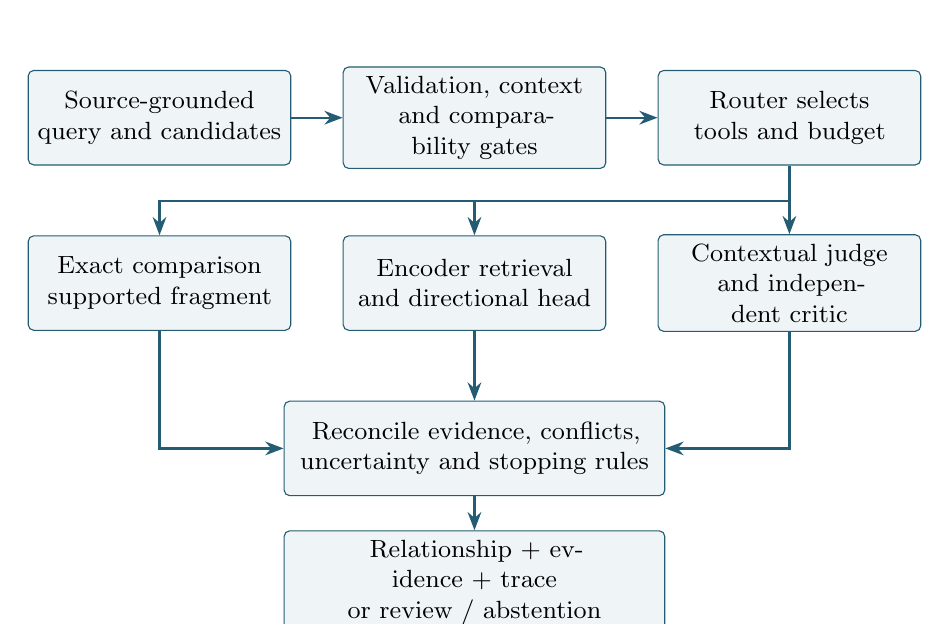
\begin{tikzpicture}[
  box/.style={draw=accent,rounded corners=2pt,fill=pale,align=center,
    text width=31mm,minimum height=12mm,font=\small},
  arrow/.style={-{Stealth},thick,draw=accent}]
\node[box](input) at (0,0) {Source-grounded\\query and candidates};
\node[box](gate) at (4,0) {Validation, context\\and comparability gates};
\node[box](router) at (8,0) {Router selects\\tools and budget};
\node[box](exact) at (0,-2.1) {Exact comparison\\supported fragment};
\node[box](encoder) at (4,-2.1) {Encoder retrieval\\and directional head};
\node[box](llm) at (8,-2.1) {Contextual judge\\and independent critic};
\node[box,text width=46mm](reconcile) at (4,-4.2) {Reconcile evidence, conflicts,\\uncertainty and stopping rules};
\node[box,text width=46mm](output) at (4,-5.9) {Relationship + evidence + trace\\or review / abstention};
\draw[arrow](input)--(gate);\draw[arrow](gate)--(router);
\draw[arrow](router.south)--++(0,-.45)-|(exact.north);
\draw[arrow](router.south)--++(0,-.45)-|(encoder.north);
\draw[arrow](router)--(llm);
\draw[arrow](exact.south)|-(reconcile.west);
\draw[arrow](encoder)--(reconcile);\draw[arrow](llm.south)|-(reconcile.east);
\draw[arrow](reconcile)--(output);
\end{tikzpicture}
\caption{Proposed runtime. Retrieval proposes comparisons; routing decides
which additional reasoning is required. A route can use several tools without
making every request execute the same fixed chain.}
\end{figure}

The input contract contains the two records, necessary parent evidence,
corpus/split identifiers, requested comparison mode, and a tool budget. A
tool output should contain a supported label or unresolved result, explicit
preconditions, field differences, cited evidence, assumptions, and a
requires-context flag. Scores must identify their meaning: cosine similarity,
uncalibrated classifier score, calibrated probability, or a deterministic
logical result are different objects.

The initial router can be a transparent rule policy. Numerical records with
matching supported quantity/context signatures may enter the exact route;
large candidate searches use the encoder; exceptions, ambiguous history,
measurement incompatibility, and unresolved scope invoke contextual review.
A learned routing policy is a later experiment requiring its own labels and
cost/quality evaluation, not a prerequisite for an auditable prototype.

\subsection{Exact Comparisons}
\label{sec:exact}

\subsubsection{Supported fragment and admission gates}
The exact route is a conservative comparator for an explicitly supported
fragment: scalar thresholds, complete intervals, supported unit conversions,
categorical predicates with controlled semantics, and simple temporal windows
with shared anchors. More complex temporal expressions, clinical
hierarchies, assay conversions, and nested Boolean conditions require
additional representation or contextual reasoning.

Before emitting an exact relationship, check entity identity, measurement
method, applicable population, units/reference basis, temporal anchor,
repetition, exceptions, negation, and Boolean scope. Numerical validity alone
does not satisfy these gates. Missing context is not a wildcard match.
An unsupported case returns a reason for escalation rather than a fabricated
exact answer.

\subsubsection{Interval algebra and directional containment}
Represent a numerical constraint by a lower endpoint, lower inclusivity,
upper endpoint, and upper inclusivity. Missing endpoints denote unbounded
directions only where the comparator actually establishes that meaning.
For example, $x>t$ becomes $(t,+\infty)$ and $x\leq t$ becomes
$(-\infty,t]$. Strict and inclusive boundaries remain distinct.

Compare the resulting allowed sets, including any complement introduced by
an exclusion rule. First check equality, then proper containment, then
disjointness, and finally genuine partial overlap. At a shared endpoint,
intersection exists only if both intervals include that point. Excluding an
interval can yield a union of two intervals; a comparator that supports only
one interval must escalate that case or implement a verified interval-union
representation. It must not drop one side of the complement.

An exact explanation should expose the transformation, for example:
``A allows $[21,+\infty)$ and B allows $[18,+\infty)$; A is a proper subset
of B.'' A witness such as age 19 can illustrate why B allows an additional
case. Such a witness is a logical example, not an actual patient or an estimate
of how many people a trial would enroll.

\subsubsection{Units, reference ranges, and time}
Use versioned, deterministic conversion rules only for commensurable
quantities. Record both the source and converted value. An absolute
concentration cannot be compared to a ULN multiple without a shared reference
value and assay context. Drug washouts expressed in half-lives similarly
require a drug-specific half-life and an approved interpretation before a
fixed-day conversion is possible.

Temporal comparison needs the event, anchor, direction, duration, and
inclusivity. ``Within 30 days before first dose'' differs from ``30 days after
the last dose.'' A rule using the lesser of 28 days or five half-lives is a
conditional duration expression, not a single fixed bound. Endpoint
tolerances and investigator exceptions should remain explicit. Repetition
requirements need a compatible observation definition and spacing rule; an
extra observation is not automatically a stricter criterion if its sampling
or allowed timing differs.

\subsubsection{Boolean scope, negation, and exceptions}
Do not assume a flat list of atoms is a complete formula. In an exclusion
$(A\land B)\lor C$, the record for A must remain conditional on B, and C
remains an alternative branch. The v1 parent/context fields preserve evidence,
but exact Boolean execution should require an explicit, reviewed expression
tree or an equally precise scoped representation. If this is unavailable,
use contextual review. An SMT solver is an optional future extension, not
evidence that the current flat schema already supports arbitrary logic.

An exception is part of the governing rule. If a disqualifying malignancy
predicate is $M$ and an allowed cured-cancer exception is $E$, the exclusion
predicate can be $M\land\neg E$ when that accurately reflects the source.
Encoding E as an independent exclusion reverses its role. Internal negation,
categorical absence, and exclusion type must be reconciled once, explicitly.

\subsubsection{Current implementation boundary}
The repository contains a starter interval comparator and deterministic-first
orchestrator. They are scaffolding for this specification. The current
comparator does not implement proper-subset direction, complete
inclusion/exclusion set semantics, or all of the context/reference gates
above. Its hard-coded confidence values are not calibrated probabilities.
The exact-route acceptance suite should therefore include boundary,
containment, complement, scope, unit, reference, and temporal cases before
the route is described as clinically reliable.

\subsection{The Encoder Model}
\label{sec:encoder}

\subsubsection{Role, input representations, and inference}
The encoder supports scalable candidate retrieval and a representation for
supervised pair prediction. Given serialized criterion text $t(c)$, produce
a unit vector
\[
 z_c=\frac{f_{\theta}(t(c))}{\|f_{\theta}(t(c))\|_2},\qquad
 s(A,B)=z_A^{\mathsf T}z_B.
\]
The text serializer is part of the experiment configuration. An initial fair
comparison supplies identical raw criterion text to all baselines. Additional
ablations can use a structured rendering or a source-plus-context rendering,
but their results should be reported as different input conditions. Preserve
comparators, units, negation, timing, reference basis, eligibility role, and
necessary qualifiers in a structured rendering. Never include gold labels,
reviewer rationales that reveal them, or held-out annotation metadata.

The planned general baseline is
\pathcode{sentence-transformers/all-mpnet-base-v2}; its model card describes
a 768-dimensional sentence representation and default truncation beyond 384
word pieces \cite{mpnet}. The biomedical baseline is
\pathcode{FremyCompany/BioLORD-2023}, which builds on MPNet with
definition/ontology-grounded biomedical training \cite{biolord}.
For each model, pin the revision and tokenizer, inspect truncation, use the
specified pooling implementation, and save normalization and input settings.
Do not silently omit a critical exception at the end of a long parent.

Retrieval excludes the query itself and, for the cross-trial task, its trial.
Every experiment declares its permitted candidate partition. Cache keys
include corpus hash, serializer version, model revision, and inference
configuration. A cached embedding matrix is invalid when any of these changes.

\subsubsection{Directional relationship head}
A shared encoder with cosine similarity cannot distinguish A-more-restrictive
from B-more-restrictive. A proposed ordered head uses
\[
 h_{AB}=[z_A;z_B;z_A-z_B;|z_A-z_B|;z_A\odot z_B;\phi(A,B)],\qquad
 p(y\mid A,B)=\operatorname{softmax}(g_{\psi}(h_{AB})),
\]
where $\phi$ contains approved structured differences and missingness flags.
This is a proposed feature design, not a selected final architecture.
Compare a simple frozen-embedding classifier against encoder fine-tuning
before adding complexity. Structural features must be derived from the input,
not gold adjudications. A high classifier score does not authorize ignoring
failed comparability gates.

\subsubsection{Supervision and training objectives}
Training data may contain equivalences, ordinary negatives, hard negatives,
and ordered anchors. Hard negatives include lexical neighbors whose polarity,
boundary, timing, or exception changes the relationship. They should not
include unlabeled pairs arbitrarily declared negative. Restrictive and
overlapping pairs remain conceptually related; treating every non-equivalent
pair as a maximally distant negative would damage useful retrieval geometry.

One training option is a supervised contrastive loss on justified positives,
an ordered classification loss, and a diagnostic ordering loss:
\[
 \mathcal L=\lambda_{\rm con}\mathcal L_{\rm con}
 +\lambda_{\rm cls}\mathcal L_{\rm CE}
 +\lambda_{\rm ord}\max\{0,m-s(a,p)+s(a,n)\}
 +\lambda_{\rm swap}\mathcal L_{\rm swap}.
\]
Here $(a,p,n)$ is an explicitly reviewed relative-similarity triple, not an
ordering inferred from restrictiveness alone. The swap term penalizes a
failure to reverse directional labels while preserving symmetric ones.
Loss weights, margin, negative sampling, early stopping, and class weighting
are selected on development data. Report learning curves and at least three
training seeds for the final trained comparison. If supervision is inadequate
or no improvement is observed, retain the strongest frozen model and report
the result.

\subsubsection{Retrieval versus interpretation}
A useful retrieval candidate can be an equivalent rule, a stricter rule, or a
clinically important contradiction. Define the relevance policy for each
retrieval experiment rather than assuming that only equivalent pairs matter.
Training can pursue broad concept retrieval while the ordered head and exact
tools distinguish clinical relationships. Evaluate both stages so a retrieval
gain does not conceal a rise in false equivalence.

\subsection{Fuzzy Clinical Reasoning: LLM Judge and Critic}
\label{sec:critic}

\subsubsection{Tasks and evidence-bounded prompts}
The contextual route handles cases where an exact interpretation is not
licensed by the supported fragment: implicit clinical language, exceptions,
severity/history distinctions, incompatible measurements, treatment settings,
or unresolved branch scope. The judge receives the ordered pair, source
excerpts, necessary parent/context, reviewed structured fields, and any
validated tool evidence. Retrieved neighboring criteria can provide precedent
only when the experimental policy allows them; they cannot establish facts
missing from the two source rules.

The prompt requests a structured answer: proposed label, direction, cited
evidence spans, field/context differences, assumptions, uncertainty reason,
and review/abstention disposition. Instructions distinguish absent evidence
from evidence of absence. The model should name a missing temporal anchor or
assay mapping rather than supply a clinically plausible one from memory.
Source text is untrusted task data: embedded instructions in a protocol or
retrieved document cannot authorize tool calls or override the task policy.

\subsubsection{Independent criticism and bounded revision}
The critic is a separate invocation that checks the proposed answer against
the original evidence and any exact-tool certificate. Its checklist covers
source support, inclusion/exclusion interpretation, negation, units and
references, interval direction, timing, exceptions, branch scope, and
unsupported assumptions. It also checks whether the label remains correct
when the input order is reversed.

The critic may accept the supported result, identify specific repairable
errors, or require abstention/reviewer escalation. One bounded revision
followed by a final evidence check is an initial policy to evaluate; repeated
self-discussion is not a substitute for missing evidence. A second call to
the same model can have correlated errors, so critic agreement is not an
independent human gold label or proof of correctness. Measure the critic's
incremental benefit with a no-critic ablation.

\subsubsection{Validation, reconciliation, and uncertainty}
Validate schema, allowed label values, valid criterion IDs, required evidence,
and quote grounding before accepting a model response. Invalid JSON, missing
decisions, corrupted text, unsupported evidence, timeouts, and refusal/error
responses are operational failures with explicit dispositions. They must not
silently become unrelated or equivalent labels.

If the judge conflicts with the exact route, first recheck the exact route's
preconditions. A mathematical result is conclusive only for its encoded
predicate; the encoding itself may be wrong or incomplete. An unresolved
conflict triggers escalation. Do not reconcile incompatible labels by taking
an unvalidated weighted average of cosine, a classifier score, and model
self-reported confidence.

Separate \emph{source ambiguity} from \emph{model uncertainty}. The former
concerns what can be established from the inputs; the latter concerns the
system's reliability in choosing an answer. Confidence calibration requires
held-out development labels. Until then, expose raw scores and categorical
reasons for review. Select any automatic-accept threshold on development
risk--coverage results, then freeze it for test evaluation.

\subsection{Trace, stopping policy, and operational behavior}
Each comparison receives a trace with ordered input IDs, corpus/source hashes,
serializer and normalization versions, tool/model/prompt versions, route
reasons, evidence, outputs, conflicts, final disposition, and human edits.
Record wall-clock latency, token usage, configured pricing date when cost is
reported, cache hits, retries, and tool errors. Store task evidence and
auditable summaries, not a claim to expose private internal model reasoning.

The prototype should have explicit budgets for candidate count, tool calls,
revision attempts, timeout, and cost. A valid exact result can stop without
an LLM call; unresolved language can stop with abstention when the evidence
is insufficient. Training and benchmarking must record these policies so
reduced cost cannot be explained by silently dropping hard cases.

\section{UI/UX Design}
\label{sec:ui}

\subsection{Clinical users and decisions to support}
\textbf{Design status: exploratory.} The interface should be shaped by task
observation and feedback from clinicians and trial staff. The following
personas are design hypotheses rather than findings from a completed user
study.
\begin{itemize}
\item A protocol investigator asks which historical rules operationalize the
same concept and how a proposed change affects restrictiveness.
\item A research coordinator needs a source-grounded explanation of a flagged
difference and a way to send it for investigator review.
\item A reviewer or methodologist needs to compare multiple protocols, record
adjudications, and export an evidence trail for a design or harmonization meeting.
\end{itemize}

The primary interface question remains the proposal's practical task: given a
current rule, which historical criteria are comparable, how do they differ,
and what evidence supports the result? Avoid presenting the tool as a
patient-screening interface when it has neither patient inputs nor validated
screening logic.

\subsection{Core interaction and information architecture}
\planned\ A three-region workspace can put a query and source context on the
left, a ranked candidate list in the center, and a selected comparison on the
right or in an expanded lower panel. A compact view should answer the clinical
question before showing implementation traces.
\begin{enumerate}
\item Select a source trial and criterion, or enter a draft rule. If draft text
is parsed, display the parsed interpretation for confirmation and mark it as
an unreviewed draft rather than part of the frozen corpus.
\item Inspect the source wording, parent, role, population, time, and provenance.
\item Retrieve candidates with filters for therapeutic area, clinical concept,
trial, source version, and comparison status. Clearly show which filters
constrain the search; exclusion of a candidate is not a clinical decision.
\item Select a candidate and inspect its relationship, the decisive
differences, supporting source spans, and any unresolved assumptions.
\item Accept, correct, or leave unresolved with a rationale. Distinguish a
human review action from a system's automatic-accept recommendation.
\item Export the reviewed comparison with source and version identifiers.
\end{enumerate}

A search result should show the candidate's source excerpt, trial, clinical
concept, and relevance score type. A relationship label appears only when
comparison has actually run. ``No results'' should distinguish restrictive
filters, no candidate match, unavailable indexes, and tool failure. A blank or
failed route must not look like a confident negative finding.

\subsection{Visualization ideas retained from the proposal}
These ideas remain candidates for the design, with implementation priority
based on clinical usefulness and feasibility.
\begin{longtable}{L{.23\linewidth}L{.42\linewidth}L{.26\linewidth}}
\toprule Concept & Useful presentation & Initial priority / limitation\\\midrule
\endhead
Side-by-side constraint comparison & Align entity, role, comparator/value, units/reference, interval, timing, repetition, qualifiers, Boolean scope, and source; annotate the decisive difference. & Highest priority. Keep source language accessible beside normalized fields.\\
Numerical allowed-region plot & Draw the two admissible sets with open/closed endpoints, intersection, and containment; label the common quantity and units. & High for supported numerical cases. Draw allowed regions after polarity handling; hide the plot when context/conversion gates fail.\\
Agent decision trace & A compact route diagram expands to tool inputs, evidence, conflicts, critic disposition, and final action. & High. Show the real executed trace, not a decorative flowchart implying uncalled tools ran.\\
Method-agreement panel & Compare lexical/encoder rankings, exact result, judge, critic, and final decision without collapsing their distinct meanings. & High. Label cosine as similarity, not probability.\\
Uncertainty and review indicator & Show supported result, needs review, or unable to determine, with a specific reason and calibrated probability only when available. & Medium. Source ambiguity and model confidence are different dimensions.\\
Similarity versus clinical relationship plot & A cohort-level plot identifies false-high and false-low similarity by reviewed label and clinical phenomenon. & Medium, after labels exist. Appropriate for results/error analysis rather than the primary comparison screen.\\
Two-dimensional retrieval map & An optional projected neighborhood colored by reviewed relationship and marked by route. & Exploratory. Projection distances are not literal clinical distances and can distort the original geometry.\\\bottomrule
\end{longtable}

\subsection{Additional clinician-oriented interface ideas}
\subsubsection{Protocol comparison matrix and review packet}
A clinician may start with two protocols rather than one criterion. A
comparison matrix could list clinical concepts as rows and protocols as
columns, highlighting matched rules, missing matches, and unresolved scope.
An unmatched rule means no supported match was found; it does not prove that
the other full protocol lacks that requirement. A review packet could export
selected comparisons, excerpts, source versions, reviewer rationale, and open
questions for a protocol-design meeting.

\subsubsection{Amendment difference view}
For two versions of one protocol, separate wording-only changes from changed
thresholds, windows, exceptions, or measurement methods. Show a proposed
direction of change only for supported comparable rules. Preserve both
versions and the amendment lineage. This is a useful future workflow, but
amendments must remain in the same family for evaluation.

\subsubsection{Source-first evidence drawer and context expansion}
Every result can open an evidence drawer with highlighted source spans, parent
statement, adjacent context, snapshot version, and registry link. Link a
clinical summary such as ``longer treatment washout'' to the exact two windows
that support it. Offer an explicit ``context not sufficient'' disposition
instead of making the reviewer search for a hidden caveat.

\subsubsection{What-if comparison sandbox}
A draft workspace could let a user change one threshold or window and inspect
the logical relationship to the original. Keep draft versions separate from
the frozen corpus, and require confirmation of a parsed rule. A numerical
witness can illustrate the set difference. Do not translate that difference
into recruitment percentages or clinical safety claims without the additional
data and validation those claims require.

\subsubsection{Disagreement and adjudication queue}
A review queue can prioritize exact/LLM conflicts, missing evidence, uncertain
scope, or method disagreement. Show why each case was queued and support
assigning a reviewer, adding an interpretation, and preserving earlier
decisions. An override requires a rationale and evidence; a corrected result
does not erase the model's original prediction from the evaluation record.

\subsubsection{Saved cohorts of comparisons and precedents}
Users may collect a set of source-backed precedents for a clinical concept,
bookmark unresolved questions, and compare the same draft against several
historical protocols. Group results by distinct trial/family so repeated
template wording does not create a false impression of broad independent
precedent. Saved sets should record filters and source versions for replay.

\subsection{Accessibility, uncertainty, and usability validation}
Use text and icons in addition to color; show full labels rather than only
red/green agreement. Support readable typography, keyboard navigation,
sortable lists, and expandable evidence without forcing a dense field table
on every user. Prefer plain clinical explanations with technical details
available on demand. Distinguish ``evidence not available'', ``not comparable'',
``system error'', and ``review pending''.

Evaluate prototype tasks with trial staff: find a supported precedent, identify
a consequential threshold or scope difference, reject an unsupported
equivalence, and complete an adjudication/export. Record task success,
time, corrections, overlooked caveats, and users' interpretation of score
labels. This is a proposed usability study; no clinician preference or
efficiency gain is assumed. A within-person comparison with and without the
tool should counterbalance task order if used to measure time savings.

\subsection{Demonstration scope and resilience}
For November 17, target the ranked list, aligned constraint view, supported
interval plot, genuine route trace, and a method-agreement view. Add a
confidence indicator only if its interpretation is defensible. By December 8,
include the error-analysis plot and a documented uncertainty/review policy.
The projected map and larger protocol matrix are optional extensions.

The live demonstration must include a success, an important failure, and a
necessary abstention. A cached mode replays the same versioned inputs and
outputs and is labeled as replay. A recording or screenshots provide a final
fallback. Before presentation, verify environment startup, corpus/index
versions, credentials, network availability, expected latency, source links,
and cached mode. The current Streamlit application is a candidate-table
placeholder, not an implemented version of this workspace.

\section{Evaluation and Comparisons}
\label{sec:eval}

\subsection{Benchmark construction and evaluation units}
Maintain separate pair-classification and retrieval evaluations. Pair
classification tests a fixed set of ordered comparisons with reviewed labels.
Retrieval tests a query and a declared pool of candidate criteria. A model can
classify supplied pairs correctly while failing to retrieve them, or retrieve
relevant concepts while confusing their relationship. Report both stages.

Use family splits before mining, preserve reversed/constructed variants in
their source partition, and keep test labels unavailable to training,
prompt design, model selection, agent memory, or retrieval of labeled
precedents. Encoding held-out candidate text for a declared test search index
is different from training on it; document the intended inductive evaluation.
Fit TF--IDF vocabulary/IDF and all learned preprocessing on training text only.
Select hyperparameters, calibration, and acceptance thresholds on development
data. Run the untouched test evaluation after those choices are frozen.

Pool candidate judgments across the proposed baselines so one encoder does
not determine the entire benchmark. Report judgment coverage, label counts,
sampling strata, and the number of queries with known relevant candidates.
Unjudged items are not automatically negatives. If the candidate pool is
incompletely judged, call recall relative to that judged pool and disclose
that it is not exhaustive corpus-wide recall.

\Needspace{12\baselineskip}
\subsection{Baseline Embedding Comparisons}
\label{sec:baselines}
\begin{longtable}{L{.22\linewidth}L{.37\linewidth}L{.32\linewidth}}
\toprule Baseline & Fixed implementation / role & Key controls\\\midrule
\endhead
Lexical & TF--IDF with lowercase word unigrams/bigrams and cosine ranking. & Fit only on training data; retain operators/negation in an audited serializer and record tokenization limitations.\\
General encoder & Frozen \pathcode{sentence-transformers/all-mpnet-base-v2}. & Pin revision, pooling, truncation and input rendering.\\
Biomedical encoder & Frozen \pathcode{FremyCompany/BioLORD-2023}. & Same candidate pool and input condition; document model-card license requirements before redistribution.\\
CReSE-informed representation & Eligibility-oriented representation/rephrasing approach, conditional on reproducible artifacts. & Distinguish an actual reproduced checkpoint from a newly implemented inspired baseline.\\
TriAlign encoder & Fine-tuned representation plus an ordered prediction head, when sufficient labels exist. & Same held-out evaluation; compare with frozen features and report training seeds.\\\bottomrule
\end{longtable}

The raw-text baseline is the simplest matched input condition. A second
condition may provide the same structured/context rendering to every method.
Do not compare a context-rich TriAlign input against context-deprived baselines
without separately identifying that input advantage. A separate relationship
classifier can be trained on each frozen embedding under the same protocol
to isolate representation quality from the value of fine-tuning.

The model inventory in configuration also lists MiniLM, BGE, and SapBERT.
They are optional candidates, not mandatory experiments or established
improvements. Add one only with a documented question, pinned revision,
supported input policy, and sufficient time to run the same evaluation.
The required initial comparison remains TF--IDF, MPNet, and BioLORD.

\subsection{Existing Eligibility Systems and Products: Research Notes}
\label{sec:systems}
The following entries are research notes for the systems named in the
proposal. Most are research methods or software artifacts, not interchangeable
commercial clinical products. No shared eight-class benchmark results or
TriAlign adapters are claimed here. Availability of a paper or repository
does not establish installation success, compatible licenses, usable model
weights, or reproduction of the published results.

\subsubsection{CReSE: eligibility recommendation and representation}
\research\ The published work introduces eligibility-criterion recommendation
from trial information and an evaluation framework using contrastive learning
and LLM rephrasing \cite{crese}. Its representation objective makes it a
relevant comparator for eligibility-specific embeddings; its native task is
not TriAlign's directional eight-label comparison.

\textbf{Proposed comparison.} If a suitable checkpoint or reproducible
training path is available, evaluate criterion embeddings on the same
retrieval pools, with any relationship head trained only on TriAlign training
pairs. Otherwise report a clearly named CReSE-inspired experiment rather
than claiming to reproduce CReSE.

\textbf{Open research items.} Identify code/checkpoints, exact preprocessing,
data access and license, and possible source-trial overlap. Determine whether
rephrasing preserves strict comparators, exclusion roles, and exceptions.
Exit artifact: an availability/reproduction note and, only if feasible, a
matched retrieval result.

\subsubsection{TrialGPT: patient-to-trial matching}
\research\ The official repository describes retrieval, criterion-level
patient eligibility matching, and trial ranking, and provides code and data
\cite{trialgptcode}. These inputs and outputs differ from comparing two
protocol criteria. Its original patient-matching labels cannot be relabeled
as TriAlign relationships without a justified task transformation.

\textbf{Proposed comparison.} Inspect its evidence-and-judgment prompt design
and implement a separately named criterion-pair adaptation if defensible.
Hold the supplied source evidence, base LLM, and allowed call budget constant
when isolating prompt/workflow differences. Compare evidence support,
abstention, latency, and cost on shared cases; preserve native results as
background rather than importing their accuracy into a TriAlign leaderboard.

\textbf{Open research items.} Pin a repository revision, identify reusable
prompts and output schemas, document all changes, and determine whether a
pair adaptation is substantive enough to warrant inclusion. The cited
clinical study remains background for the original task \cite{trialgpt}.

\subsubsection{EligMeta: eligibility-aware evidence synthesis}
\research\ EligMeta connects trial discovery and eligibility-aware
meta-analysis. The paper separates LLM-generated rules/parsing from
deterministic logic, weighting, and statistical pooling \cite{eligmeta}.
Its relevant overlap is eligibility alignment and reproducible execution;
TriAlign does not implement its pooled-outcome estimand.

\textbf{Proposed comparison.} Investigate whether an exposed alignment
component can operate on the common source-grounded cases. If not, compare
architectural choices and a documented adaptation of its rule/parse/execute
pattern. Never compare TriAlign pair macro-F1 directly to meta-analysis
effect estimates or literature-selection recovery.

\textbf{Open research items.} Verify code and artifact access, alignment
granularity, treatment of exceptions and absent fields, and compatibility of
its similarity output with categorical relationships. Determine a fair
matched-case input/output contract before implementing an adapter.

\subsubsection{SatIR: constraint-satisfaction retrieval}
\research\ SatIR formulates trial matching using explicit SMT constraints
and scalable relational-algebra retrieval. The inspected paper is arXiv
version 4 and links an implementation \cite{satir,satircode}. Its native
problem is profile-to-trial retrieval rather than ordered criterion-pair
labeling.

\textbf{Proposed comparison.} Study whether its constraint representation
can support a restricted, reviewed pair-comparison fragment. Equality,
containment, and separation can be investigated through satisfiability of
set-difference/intersection formulas, provided both predicates and a common
universe are faithfully encoded. A solver's answer does not validate the
LLM translation that produced the formula.

\textbf{Open research items.} Record ontology assumptions, missing-data
policies, supported temporal/Boolean expressions, source translation
errors, and installation dependencies. Report unsupported coverage together
with correctness on supported cases. Keep retrieval-system reproduction
separate from a newly written logical pair adapter.

\subsubsection{VERDICT: accountable decisions and rationales}
\research\ VERDICT translates constraints and decision policies into SMT
and uses SMT/MaxSMT reasoning to support explicit assumptions and pivotal
conditions. It evaluates groundedness, consistency, and counterfactual
self-faithfulness in clinical-trial matching \cite{verdict}. The inspected
paper links code/prompts in the Stanford OVAL repository \cite{satircode}.

\textbf{Proposed comparison.} Adapt its rationale-oriented questions:
which source facts support the relationship, which assumptions are required,
and what supported change would alter the decision? Test whether a stated
pivotal condition actually changes a recomputed result. Treat these as
additional audits of TriAlign explanations, not automatic proof that an
explanation is clinically correct.

\textbf{Open research items.} Identify reusable policy/solver interfaces,
the boundary between facts and assumptions, coverage of conditional
exceptions, and the cost of faithful translation. A common-case adapter must
declare every modification to its native decision task.

\subsubsection{EC-RAFT: retrieval-augmented eligibility generation}
\research\ EC-RAFT generates eligibility criteria from trial titles and
descriptions using retrieval-augmented fine-tuning. Its paper identifies
Llama-3.1-8B-Instruct as the base model and links released code \cite{ecraft}.
Generation quality is a different task from pair relationship prediction.

\textbf{Proposed use.} Treat EC-RAFT as adjacent authoring research. It may
inform a future draft-criterion workflow or supply separately marked
constructed examples after source/clinical review. Generated criteria are
not automatically valid training labels or clinical precedents.

\textbf{Open research items.} Check the generation/evaluation interface,
retrieval-corpus overlap, and preservation of numerical and exception scope.
Report any generation experiment separately from the main retrieval and
relationship benchmark. It should not displace the mandatory matched-task
baselines.

\subsubsection{Common research-note template and comparison decision}
For each system, maintain primary citation, inspected version/date, native
task, input/output schema, artifact/license status, reproducible execution
status, proposed adapter, task mismatch, expected cost, and comparison
decision. Classify the outcome as: direct matched-task baseline; explicitly
adapted common-case experiment; architectural/failure-mode comparison; or
out of scope. Commercial products can be added later with the same template
if the team identifies a specific accessible product and evaluation pathway.
Do not invent a capability matrix from marketing claims or compare unavailable
systems using fabricated results.

\subsection{Agent comparisons and ablations}
The main agent experiment compares an LLM-only judge, an always-run fixed
chain, and routed TriAlign on the same supplied pairs, evidence, model
versions, and output contract. Include an exact-only route with supported-case
coverage where useful. Report both accuracy and expenditure; an expensive
always-run system can improve accuracy while being less efficient.

Ablations isolate hard negatives, human corrections, normalization/context
input, structured features/checks, critic calls, and targeted sampling.
Change one component at a time where possible and state interactions when
several components change. Routing evaluation should include selection errors,
missed opportunities to stop exactly, unnecessary LLM calls, and unresolved
conflicts. Do not score an abstaining exact-only system solely on its easy
resolved subset and compare that number to full-coverage models.

\subsection{Metrics, uncertainty, and statistical reporting}
\begin{longtable}{L{.22\linewidth}L{.40\linewidth}L{.29\linewidth}}
\toprule Evaluation target & Measures & Interpretation controls\\\midrule
\endhead
Retrieval & Precision/recall@$k$, MRR, equivalence-specific retrieval, reviewed anchor ordering. & State relevance definition, candidate/judgment pool, query denominator and judgment coverage.\\
Pair relationships & Eight-class macro-F1, per-class precision/recall, confusion matrix, directional F1 and swap consistency. & Keep class imbalance and asymmetric labels visible; report abstentions separately.\\
Clinical phenomena & Error counts/rates for thresholds, negation, units/references, timing, repetition, history, exceptions and compounds. & Give numerator/denominator and account for multi-tag cases.\\
Uncertainty & Calibration diagrams, Brier score where probabilities are defined, risk--coverage, inappropriate automatic acceptance, escalation/abstention errors. & Calibrate on development data; model self-report is not validated probability.\\
Evidence and explanation & Supported-claim rate, missing-condition errors, source-span support, contradiction and pivotal-condition checks. & Correct label and grounded rationale are distinct outcomes.\\
Workflow & Reviewer time and corrections, end-to-end latency, tool/LLM calls, tokens, cost, cache hits, failures. & Use matched tasks and comparable budgets; show live and cached execution separately.\\\bottomrule
\end{longtable}

At automatic-accept threshold $t$, define coverage as the fraction of all
evaluated cases accepted automatically and selective risk as the error rate
among those accepted. Report how many ambiguous cases are appropriately
escalated and how many answerable cases are unnecessarily deferred.
Uncertainty estimates should preserve trial-family dependence. Use paired
method comparisons and family-aware resampling; a cross-trial pair touches
two families, so an ordinary independent-pair bootstrap is not sufficient.
One option is to resample held-out families and retain/weight pairs through
their endpoint-family memberships, applying the same resample to all methods.
Predeclare the chosen scheme and summarize sensitivity rather than implying
that one simple bootstrap removes every dependency.

Report at least three seeds for trained models, effect sizes and intervals,
sample sizes, family counts, and the limits of a 100-trial convenience cohort.
Separate natural from constructed challenges. The final report must show
representative false-high/false-low similarity, a routing or interpretation
failure, and a necessary abstention alongside successes.

\appendix
\section{Implementation, Delivery Milestones, and Reproducibility}
\label{sec:delivery}

\subsection{Repository boundary and work ownership}
The repository currently provides criterion/pair schemas, workbook and
Parquet adapters, candidate generation, family-splitting utilities, a TF--IDF
runner, a lazy Sentence Transformers wrapper, a starter exact comparator, a
deterministic-first orchestrator, and a placeholder review application.
These interfaces do not establish that fine-tuning, contextual judging,
calibration, full family-aware command-line splitting, or the proposed UI
have been implemented. The pair generator's unordered ID and the
split/comparator integration must be reconciled with this specification
before benchmark production.

\begin{longtable}{L{.20\linewidth}L{.35\linewidth}L{.36\linewidth}}
\toprule Workstream & Jonathan Ma (JM) & Jiatong Gao (JG)\\\midrule
\endhead
Data and benchmark & Source release, normalization, family mapping, pair guide, construction, labels, adjudication, source validation and manifests. & Consume frozen development inputs and report interface/data issues without rewriting gold labels.\\
Models and agent & Define comparison semantics, metrics, and case-level evaluation requirements. & Implement and run TF--IDF/MPNet/BioLORD, routing/tools/critic, traces, comparison adapters where feasible, and UI-facing outputs.\\
Evaluation & Freeze splits/labels, audit directionality and reported case evidence. & Save predictions, rankings, runtime/cost logs, ablations and model/configuration artifacts.\\
Submission & Data/evaluation documentation, test-case index, provenance and contribution record. & Baseline/agent implementation documentation, reproducible execution, prompts, traces and UI assets.\\\bottomrule
\end{longtable}

Shared work includes reviewing changes, agreeing on contracts, inspecting
successes and failures, rehearsing demonstrations, integrating the report,
and recording contributions by artifacts and commits. JM retains authority
over gold labels and evaluation-set changes; JG owns baseline and orchestrator
implementation. Proposed independent second annotation should be arranged
without confusing an annotator's input with final adjudication authority.

\subsection{Milestone 1: October 20 presentation, completed}
The first presentation introduced the clinical problem, source-data pipeline,
100-trial cohort, structured comparison, embeddings, agent design, and initial review work.
Recorded feedback requested eligibility-focused system comparisons and
consideration of sharing a documented criterion subset with another
clinical-trials group working with JEV. Any such sharing preserves public
source provenance, intended use, and evaluation-label separation.

\subsection{Milestone 2: November 17 presentation}
The format is 15 minutes plus 5 minutes of Q\&A. The presentation must cover
objective, dataset, workflow, preliminary positive and negative results, a
live UI, limitations, and next steps.
\begin{enumerate}
\item JM delivers the frozen criterion release and data dictionary, approves
the pair-labeling contract, establishes family splits before pairing, and
provides a versioned pilot with evidence and directional consistency checks.
\item JG runs the three required frozen baselines on common inputs, prepares
TrialGPT/EligMeta capability and adaptation notes, implements an auditable
prototype router, and compares it with LLM-only/fixed-chain execution on
the supplied development pairs.
\item Together, integrate ranked candidates, source/context, aligned
constraints, supported numerical plots, real route traces, and cached replay.
Save at least one success and one meaningful failure; demonstrate abstention
when needed.
\end{enumerate}
The v1 criterion freeze is complete. Pair labels and implementation/evaluation
artifacts remain subsequent deliverables. An approximately 200--300-pair pilot
is an optional planning target, not an existing benchmark or a guaranteed
class-balanced sample. If fine-tuning is not ready, report frozen baselines
rather than an unvalidated training run.

\subsection{Milestone 3: December 8 final presentation}
The format is 20 minutes total for presentation, demonstration, and Q\&A.
The final package for this milestone includes the frozen corpus/labels and
family splits; reproducible baseline and agent configurations; trained-model
results if justified; comparative evaluation, ablations and uncertainty
analysis; documented positive/negative cases; and stable live/cached demos.

JM finalizes and validates the benchmark and all denominators. JG completes
baseline runs, agent routing/reconciliation/critic/escalation, feasible
external-system adapters, and UI integration. Freeze dataset, model, prompt,
normalization, routing and calibration versions before the untouched test
run. Do not change gold labels to accommodate method errors; genuine source
corrections require a transparent versioned amendment.

\subsection{Milestone 4: December 22 report and submission}
The report is 5--8 pages excluding references and permitted appendices. This
technical document is supporting material and is not constrained to that
report length. The report should cover the clinical objective; source/final
data and normalization; AI/agent workflow; benchmark and statistical methods;
results and important failures; limitations and future improvements; and
individual contributions.

The accompanying release should contain source data or a reconstruction
manifest; criterion/pair manifests and family/split files; labeling guide and
adjudication provenance; code and prompts; model/index/configuration versions;
per-case inputs, predictions, evidence, traces and review outcomes; summary
tables generated from saved outputs; and reproducible training instructions
or model artifacts. The README must cover installation, dependencies, API
access, execution, expected outputs, reproduction and troubleshooting.

Verify a clean-environment execution of data loading, baseline inference,
agent comparison, evaluation and demonstration. Link every report example to
its frozen case and source evidence. Record cache behavior and the limits of
reproducing stochastic external-model outputs. Freeze a tagged submission
archive after the contribution statements and numerical claims are audited.

\subsection{Risks, mitigations, and definition of done}
\begin{longtable}{L{.25\linewidth}L{.67\linewidth}}
\toprule Risk & Mitigation and reporting requirement\\\midrule
\endhead
Insufficient pair labels & Prefer a smaller well-supported benchmark, preserve uncertainty, seek independent annotation of a subset, and report learning curves.\\
Extraction/normalization errors & Preserve raw evidence and correction lineage; version changes; escalate unsupported reference/context assumptions.\\
Leakage & Map families before mining; group amendments/templates/variants; restrict fitting, prompt development and labeled retrieval memory to approved partitions.\\
No fine-tuning or routing gain & Report negative findings and ablations; retain the strongest justified frozen configuration.\\
Unfair external comparisons & Require a matched output contract or identify the work as an adaptation/architectural comparison; do not combine incomparable native metrics.\\
Uncalibrated confidence & Label scores accurately; select thresholds on development data; report coverage and error together.\\
Live/API failure & Use bounded retries, explicit error states, cached replay, and a rehearsed recording fallback.\\
Clinical overinterpretation & Keep criterion-level inference, logical witnesses, and protocol precedent distinct from patient screening, population prevalence and causal conclusions.\\\bottomrule
\end{longtable}

Done means another person can reconstruct the approved data release, run the
documented workflow, reproduce principal results within stated tolerances,
inspect every evaluation case and source, operate the demonstration, and
distinguish source evidence, model proposals, human adjudication, and
unresolved outcomes. Completing the interface or producing a high aggregate
score alone does not satisfy that definition.

\clearpage
\begin{thebibliography}{99}
\bibitem{mpnet} Sentence Transformers. \emph{all-mpnet-base-v2 model card}.
\url{https://huggingface.co/sentence-transformers/all-mpnet-base-v2}.
\bibitem{biolord} FremyCompany / F. Remy et al. \emph{BioLORD-2023 model card}.
\url{https://huggingface.co/FremyCompany/BioLORD-2023}.
\bibitem{crese} S. Kim et al. \emph{CReSE: Benchmark Data and Automatic Evaluation Framework for Recommending Eligibility Criteria from Clinical Trial Information}.
Findings of EACL, 2024. \url{https://aclanthology.org/2024.findings-eacl.149/}.
\bibitem{trialgpt} Q. Jin et al. \emph{Matching patients to clinical trials with large language models}.
Nature Communications, 2024. \url{https://doi.org/10.1038/s41467-024-53081-z}.
\bibitem{trialgptcode} NCBI NLP. \emph{TrialGPT: official code and data}.
\url{https://github.com/ncbi-nlp/TrialGPT}.
\bibitem{eligmeta} Y. Zhao, Z. Zhang, and Y. Xu.
\emph{Eligibility-Aware Evidence Synthesis: An Agentic Framework for Clinical Trial Meta-Analysis}.
arXiv:2604.02678v1, 2026. \url{https://arxiv.org/abs/2604.02678v1}.
\bibitem{satir} Z. Zhou et al. \emph{SatIR: Scalable High-Recall Constraint-Satisfaction-Based Information Retrieval for Clinical Trials Matching}.
arXiv:2604.08849v4, 2026. \url{https://arxiv.org/abs/2604.08849v4}.
\bibitem{verdict} Z. Zhou et al. \emph{Accountable AI with Grounded, Faithful, Consistent, Actionable Rationales: A Case Study in Clinical Trial Matching with VERDICT}.
arXiv:2609.03366v1, 2026. \url{https://arxiv.org/abs/2609.03366v1}.
\bibitem{satircode} Stanford OVAL. \emph{Clinical Trial Matching: SatIR and VERDICT implementation}.
\url{https://github.com/stanford-oval/clinical-trial-matching}.
\bibitem{ecraft} N. Lekuthai et al. \emph{EC-RAFT: Automated Generation of Clinical Trial Eligibility Criteria through Retrieval-Augmented Fine-Tuning}.
Findings of ACL, 2025. \url{https://aclanthology.org/2025.findings-acl.491/}.
\bibitem{chia} F. Kury et al. \emph{Chia, a large annotated corpus of clinical trial eligibility criteria}.
Scientific Data 7, 281, 2020. \url{https://www.nature.com/articles/s41597-020-00620-0}.
\end{thebibliography}
\end{document}
